\documentclass[a4paper]{article}
\usepackage{titling}
\usepackage{amsmath}
\usepackage{mathtools}
\pagenumbering{gobble}
\usepackage{graphicx}
\usepackage{hyperref}
\usepackage[bottom]{footmisc}
\usepackage{booktabs}
\usepackage{sectsty}
\usepackage{wrapfig}
\sectionfont{\centering}
\usepackage{array}
\usepackage{subfig}
\usepackage{paralist}
\usepackage{verbatim}
\usepackage{subfig}
\usepackage{algorithm}
\usepackage{algpseudocode}
\usepackage{fancyvrb}
\usepackage{multirow}
\usepackage{rotating}
\usepackage{pgfplots}
\usepackage{wrapfig}
\pgfplotsset{width=4cm,compat=1.9}
\usepackage{fancyhdr}
\usepackage{float}
\usepackage{hyperref}
\usepackage{amsfonts}
\usepackage[utf8]{inputenc}
\usepackage[scaled]{helvet}
\usepackage{titlesec}
\usepackage{lipsum}
\usepackage[margin=0.5in]{geometry}
\setlength{\droptitle}{-5em}
\renewcommand\familydefault{\sfdefault} 
\usepackage[T1]{fontenc}
\author{}
\date{}
\title{MCMC Storage Guide \vspace{-5em}}


\begin{document}
\maketitle
\section*{\centering\textnormal{Assessing the Computational Efficiency of Different Approaches}}
\noindent The aim of this simulation study is to offer technical guidance regarding the storage of large data frames containing samples obtained using Markov Chain Monte Carlo (MCMC) methods. The samples are of the form $(\theta^{(1)}, \dots, \theta^{(m)})$, where $\theta = (\theta_1, \dots, \theta_p)$. The resulting data frame has dimensions $m \times p$, where $p \approx 10$ and $m \approx 10^8$. \\

\noindent The proposed approaches are the following: \\
(1) data frame row-wise: Create a m$\times$p data frame of NA values; fill each row sequentially.\\
(2) data frame column-wise: Create a p$\times$m data frame of NA values; fill each column
sequentially and transpose the resulting data frame.\\
(3) matrix row-wise: Create a m$\times$p matrix of NA values; fill each row sequentially and
then convert to a data frame.\\
(4) matrix column-wise: Create a p$\times$m matrix of NA values; fill each column sequentially
then transpose the matrix and convert to a data frame.\\

\noindent A simulation study is performed for each of the approaches above for $m = 10$ and $p = 10^7$, where the rows or columns respectively are filled sequentially with randomly generated samples from the standard Normal distribution, after pre-allocating a data frame or matrix with the appropriate dimensions, filled with NA values. It is worth noting that for any computations including data frames, the 'data.table'\footnote{More information about the package 'data.table' can be found in "https://cran.r-project.org/web/packages/data.table/".} package is employed instead of the corresponding base R function 'data.frame'. This is because data frames are typically characterised by sub-optimal computational efficiency and significant memory demands for very large dimensions. On the contrary, 'data.table', an extension of the base R's data.frame, is designed to optimise both speed and memory usage for big datasets. The results can be seen in Figure \ref{fig1}. It is clear that the data-frame focused methods (1) and (2) are significantly slower than the matrix-focused ones. More specifically, methods (1), (2), (3) and (4) required approximately 2.6, 4, 1.4 and 1.2 minutes to complete. Consequently, it's reasonable to exclude methods (1) and (2) from consideration for the problem at hand.\\

\begin{figure}[H]
\caption{}
\centering
\label{fig1}
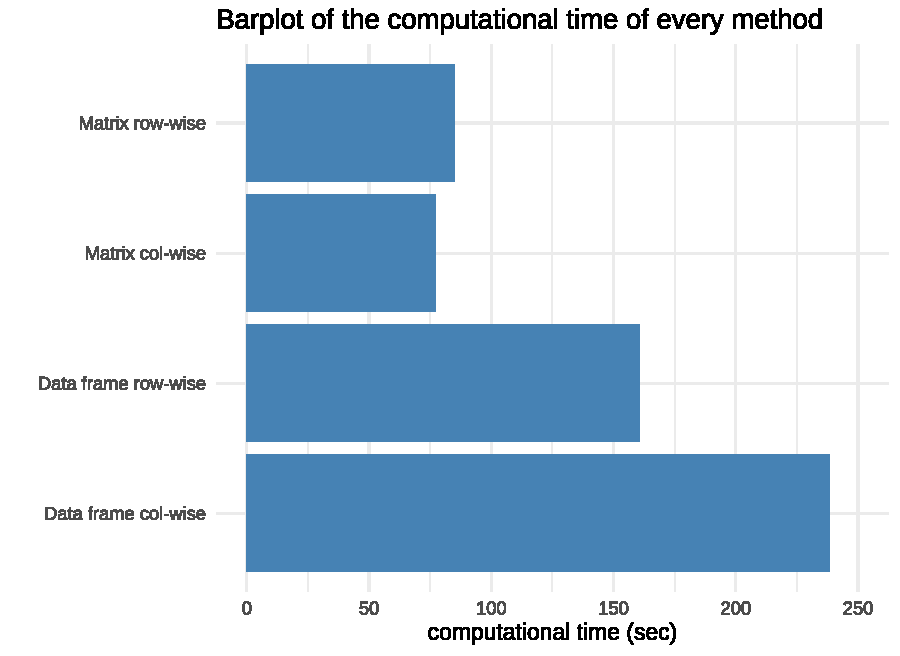
\includegraphics[width = 0.6\textwidth]{03-01-barplot.pdf}
\end{figure}

\noindent As the remaining matrix-focused methods demonstrate almost identical computation times for $p = 10^7$, further investigation is required; the simulation study is thus repeated for the two methods, this time for $p = 10^8$. The computation time for the column-wise and row-wise method is approximately 20 and 7 minutes respectively. Thus, filling the matrix by row is more than 2 times faster than filling it by column \& then transposing it, for $p = 10^8$. Based on the observed results, a definitive conclusion can be drawn that the row-wise matrix method (3) is the fastest among the options examined.\\

\noindent It's important to acknowledge that computation times may significantly vary across different devices and even between runs on the same device. Hence, the focus of this guide is not as much on the computation time values as it is on the relative computation times of each method investigated. Additionally, the implementation of the actual MCMC method is likely to require an increased computation time, depending on the complexity of the method employed, as well as the dependence present between successive runs (and thus rows of the resulting data frame) that is a common characteristic of such methods.\\

\end{document}


